\mychapterfoot{Introduction\label{ch:1}}

\footnotetext{Elements of this chapter are based on work completed in Ref.~\cite{Deshmukh2015a}.}

\epigraph{\textit{``Nevertheless, the design method is as inherent to the design process as the scientific method is to scientific exploration.''}}{\textmd{R. J. McCrory} \cite[p.~12]{McCrory1966a}}

% start of content
The advancement of many engineering systems relies on novel design methodologies, design formulations, and design representations among other parts.
In this work, we consider three broad design domains: \textit{architecture}, \textit{plant}, and \textit{control}.
These domains cover most of the potential design elements of an engineering system (and in particular, of dynamic systems, or systems whose behavior evolves through time).
Allowing design flexibility (where appropriate) in all three of these domains is the first step for formulating, solving, and understanding novel and innovative design problems.
Furthermore, achieving design automation in these types of problems requires adequate theory and tools to support such considerable scope and complexity. 

\section{Introductory Example\label{sec:ch1:example}}

We begin with an introductory design problem that includes decisions that can be classified under the architecture, plant, and control design domains.
This short example will help build some initial intuition for the types of design problems considered here.

\begin{figure}
\centering

\includegraphics[width=0.4\textwidth]{../ch1/figures/robotcontrol_a.pdf}
\caption{Task description in the robotic manipulator example.\label{fig:ch1:robotcontrol_a}}
\end{figure}

% new paragraph
Consider a pick-and-place task shown in Fig.~\ref{fig:ch1:robotcontrol_a} (move an object from one place to another and return) that will be performed by a robotic manipulator (a device that can perform tasks without direct human interaction) \cite{Spong2005a}.
There are a number of ``robots'' that can perform such a task.
A few of these forms or architectures are shown in Fig.~\ref{fig:ch1:robotarch}.
Figure~\ref{fig:ch1:robotarch_a} displays a two-link serial architecture.
An alternative architecture could have an additional link placed in series as is shown in Fig.~\ref{fig:ch1:robotarch_b}.
Links can be combined in a variety of ways to create new architectures such as the four-link parallel manipulator in Fig.~\ref{fig:ch1:robotarch_c}.
Additional components or building blocks can be added to the architectures such as the triangular plate in Fig.~\ref{fig:ch1:robotarch_d}.
There are other decisions to be made with respect to the architecture including the joints that will be active (i.e.,~an actuator is present so a torque can be directly applied to the joint).
The potential actively actuated joints are represented by red arrows in Fig.~\ref{fig:ch1:robotarch}.
From this discussion, the essence of the architecture design decisions is the selection of the components and their connectivity.

\begin{figure}
\centering
\begin{subfigure}[t]{0.22\textwidth}
\centering
	
\includegraphics[scale=1]{../ch1/figures/robotarch_a.pdf}
    \caption{Two-link serial.\label{fig:ch1:robotarch_a}}
\end{subfigure}%
\begin{subfigure}[t]{0.22\textwidth}
\centering
	
\includegraphics[scale=1]{../ch1/figures/robotarch_b.pdf}
    \caption{Three-link serial.\label{fig:ch1:robotarch_b}}
\end{subfigure}%
\begin{subfigure}[t]{0.25\textwidth}
\centering
	\includegraphics[scale=1]{../ch1/figures/robotarch_c.pdf}
    \caption{Four-link parallel.\label{fig:ch1:robotarch_c}}
\end{subfigure}%
\begin{subfigure}[t]{0.31\textwidth}
\centering
	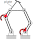
\includegraphics[scale=1]{../ch1/figures/robotarch_d.pdf}
    \caption{Four-link with a plate.\label{fig:ch1:robotarch_d}}
\end{subfigure}%
\caption[Some candidate robot manipulator architectures]{Some candidate robot manipulator architectures (red arrow indicates active joints).\label{fig:ch1:robotarch}}
\end{figure}

% new paragraph
Some potential plant design variables for this problem are shown in Fig.~\ref{fig:ch1:robotplant}.
The link length, cross-section geometry, and ground spacing are all geometric plant variables.
The spacing of the ground joints relative to point $A$ in Fig.~\ref{fig:ch1:robotcontrol_a} could also be considered plant variables.
All of these design variables are time-independent and related to the physical form of the manipulator.
The distribution of the plant variables can vary depending on the architecture considered.
If we use the two-link manipulator in Fig.~\ref{fig:ch1:robotarch_a}, then there will be only two length variables versus the four length variables associated with the four-link manipulator in Fig.~\ref{fig:ch1:robotarch_c}.

\begin{figure}
\centering
\begin{subfigure}[b]{0.33\textwidth}
\centering
	\includegraphics[height=0.5in]{../ch1/figures/robotplant_a.pdf}
    \caption{Link length.\label{fig:ch1:robotplant_a}}
\end{subfigure}%
\begin{subfigure}[b]{0.33\textwidth}
\centering
	
\includegraphics[height=0.7in]{../ch1/figures/robotplant_b.pdf}
    \caption{Cross-section geometry.\label{fig:ch1:robotplant_b}}
\end{subfigure}%
\begin{subfigure}[b]{0.33\textwidth}
\centering
	\includegraphics[height=0.8in]{../ch1/figures/robotplant_c.pdf}
    \caption{Ground spacing.\label{fig:ch1:robotplant_c}}
\end{subfigure}%
\caption{Plant variables in the robotic manipulator example.\label{fig:ch1:robotplant}}
\end{figure}

% new paragraph
The control design could involve the specification of the torque trajectories at the active joints such that the manipulator performs the pick-and-place task shown in Fig.~\ref{fig:ch1:robotcontrol_b}.
These are time-varying signals that could be chosen such that the minimum amount of time or energy is used.
The control design variables directly govern the behavior of the dynamic system.

\begin{figure}
\centering
	
\includegraphics[width=0.35\textwidth]{../ch1/figures/robotcontrol_b.pdf}
    \caption{Joint control trajectories in the robotic manipulator example..\label{fig:ch1:robotcontrol_b}}
\end{figure}

% new paragraph
It is not uncommon for each design domain to be treated separately.
For example, the architecture may be assumed to be fixed while either the plant or control is developed.
Recent work has considered combined plant and control design and this system-focused approach led to low energy consumption solutions \cite{Allison2013d}.
Considering all three of the design domains could further lead to breakthroughs in performance and completely innovative systems.
There are some potential challenges with solving this design problem including the determination of what architectures to consider, developing models for each considered architecture, and solving an appropriate optimization problem for each architecture to properly evaluate its performance.

\section{Three Design Domains\label{sec:ch1:domains}}

In this section, we will discuss the classification of the three design domains.
The purpose of these classifications is to help conceptualize what can we change and how can we handle these decisions in system-level design.

%----------------------------------------------------------
\subsection{Architecture\label{sec:ch1:architecture}}

In the engineering design context, architecture is defined as the elements contained within a system and their relationships \cite{Crawley2004a}.
An architecture design problem seeks to optimize some performance measure subject to the necessary constraints by determining both the distribution of the elements and their relationships in the system.
A complementary use of the architecture representation is during the design process (see Sec.~\ref{sec:ch1:process}) where the elements and their relationships may change for reasons other than optimization of the system's performance.
The term ``element'' is a very generic but appropriate term as the elements in an architecture can be very different.
Some dissimilar types of architecture elements include:
\begin{itemize}[noitemsep]
\item Choosing between two elements with similar function but differing properties such as motor $A$ vs. motor $B$ from a manufacturer's catalog
\item Choosing elements with different functions such as a spring vs. a damper
\item Choosing elements with different assumptions/forms such as an active vs. semi-active actuator, or feedback controller vs. open-loop controller
\item Choosing elements with different levels of model fidelity such as a linear spring vs. a nonlinear, finite element-based spring
\end{itemize}

It is important to consider that not all architecture elements are meant to be strict design decisions.
For example, seeking the best performing architecture by varying elements with similar function but different levels of model fidelity is not particularly useful.
Therefore, a key point is that an architecture representation used during the design process does not need to be the final, realizable architecture to still be useful.
There are advantages in using different levels of design representation which will be discussed more in Sec.~\ref{sec:ch1:process}.
However, the broad definition of architecture used here encompasses the whole of an engineering system and its design representation.

% new paragraph
Component is a common alternative term for element (and will be used frequently throughout this dissertation).
Often, an architecture is made up of a particular set of components chosen from a set of discrete choices or a catalog.
Components in the catalog may be homogeneous (all the same) or heterogeneous (different).
The relationships between the elements of the architecture can be frequently captured by a graph \cite{Herber2017a}.
These relationships, or connections, could be physics-based or general information sharing.
From these definitions, we see that architecture design primarily involves the determination of discrete concepts (rather than the primarily continuous variables used in the remaining two design domains).

% other names
An alternative term for architecture is topology.
Topology more commonly refers to the connections between similar elements, while architecture tends to focus on the specifics.
For example, consider a series-parallel topology for an electrical circuit.
Traditionally, such a classification implies that replacing a particular component (e.g.,~swapping a capacitor for an inductor) in the circuit would still have the same topology.
There is even a particular element type that forgos the direct specification of the component known as the general impedance element. 
However, there are alternative definitions would classify these as different topologies.
Another domain where topology is frequently used is in structural optimization \cite{Bendsoe2004a, Lohan2016c}.
In these types of architecture design problems, the elements are typically homogeneous (e.g.,~all are bars in the truss with the same type of area shape), so it does fit the definition of the connections between similar elements.
Throughout this dissertation, both may still be used interchangeably even though this delineation between architecture and topology might be useful.

% examples
There are many architectures with heterogeneous components, such as electrical circuits \cite{Macmahon1994a, Lomnicki1972a, Isokawa2016a,manuscript-pm-circuits}, hybrid powertrains \cite{Bayrak2016a}, vehicle suspensions \cite{Herber2017a}, gear trains \cite{Pennestri2015a, Castillo2002a}, and biological networks \cite{Ma2009a} that are represented by colored graphs where the colors (or labels) are the component types.
There are a large number of geometric architecture problems such as the design of trusses \cite{Bendsoe2004a}, heat spreaders \cite{Lohan2016c}, and soft robotics \cite{Cheney2013a}.
These problems sometimes have homogeneous elements, but a few have heterogeneous elements such as in soft robotics where the material at different locations can have a different behavior \cite{Cheney2013a}.
Sometimes, the architecture problem can be approximated with a continuum relaxation, such as with the solid isotropic material with penalization algorithm for structural optimization \cite{Bendsoe2004a, Lohan2016c}.
However, the final solution still needs discrete values to define a realizable architecture.

%----------------------------------------------------------
\subsection{Plant\label{sec:ch1:plant}}

The plant design is defined by variables that are generally regarded as time independent.
Often this implies physical variables such as geometry, but may be other types such as spring stiffness (a lumped quantity).
Sometimes the distinction is made when comparing between control and plant. Plant (sometimes called the artifact in this domain) are the quantities fixed during the control design. 
For example, the variables that can modify the dynamic equations without any control present would represent the plant.

% new paragraph
Frequently, the variables are continuous scalars, but other types are possible. 
Examples of continuous scalars plant variables include the lengths of the links in a robotic manipulator \cite{Allison2013d} or the cross sectional area of truss elements \cite{Bendsoe2004a}.
The distributed thickness of a beam could be a part of the plant design (an infinite-dimensional plant variable) \cite{Chilan2017a}.
Discrete variables are also possible, such as the number of teeth in a gear \cite{Budynas2014a}.

%----------------------------------------------------------
\subsection{Control\label{sec:ch1:control}}

Control seeks to govern directly the behavior of a dynamic system, i.e.,~one which evolves through time.
Unlike the other two design domains, control is frequently considered more adjustable for different tasks or conditions, i.e.,~one system may have different control schemes for different scenarios.

Generally speaking, there are two types of control paradigms: closed loop and open loop.
In \glsfirst{CLC}, there is some type of feedback mechanism where the current state of the system is considered when making decisions about the next action to take.
In \glsfirst{OLC}, there is no feedback mechanism.
With no feedback mechanism, open-loop control design variables are typically entire trajectories.
An example of an OLC variable is the torque trajectory for a rotatory actuator in a robotic manipulator \cite{Allison2013d}.
For closed-loop control, gains or other variables that modify aspects of the feedback mechanism could be considered the control design.
An example of CLC is in the infinite-horizon linear-quadratic regulator with full state feedback \cite{Liberzon2012a}.

%----------------------------------------------------------
\subsection{Ambiguity in These Delineations\label{sec:ch1:}}

While descriptions were provided for each of the three design domains, there is still some ambiguity on how to provide the appropriate classifications.
There are a number of potential reasons for this vagueness.

% new paragraph, engineers
One of the primary reasons may simply be legacy design paradigms that treat certain parts of the design as separate \cite{Allison2014a}.
System engineers may tackle the architecture design while the mechanical and control engineers deal with the plant and control designs, respectively (and what is in their domain is decided by some form of management).
Therefore, the classification of the design variables may be along the lines of what is traditionally expected for the particular type of engineer to handle during the design process.
In a system-level design approach, as is preferred in this work, this type of classification is not needed as all domains are considered uniformly.

% new paragraph, optimization
Another type of delineation is based on variable types.
Architecture design variables are discrete.
The plant consists of continuous, time-independent variables and the control is infinite-dimensional trajectories.
This classification scheme has the advantage of utilizing techniques specifically created to handle each of the variable types.
However, the discussion above for each design domain demonstrated that the domains contain variables of variety types.
In a similar way, the general theory or tools may be developed to handle certain parts of the design domains which may provide their own classifications (e.g.,~multidisciplinary design frameworks \cite{Allison2014a}).

% new paragraph, approximations
Another difficulty comes when the approximations or better representations of design variables in one domain are frequently  classified in another domain.
Consider the following examples where a design decision in one domain is approximated in another design domain:
\begin{itemize}
\item Architecture $\to$ plant: the solid isotropic material with penalization approximation in structural optimization \cite{Bendsoe2004a, Lohan2016c}

\item Architecture $\to$ control: assuming a particular feedback controller form for the power take-off in wave energy conversion so that standard control-design techniques can be applied rather than selecting a specific power take-off architecture \cite{Falnes2002a}

\item Plant $\to$ architecture: using only preferred discrete component values in a circuit (e.g.,~E12 series) rather than continuous values for the inductance and capacitance \cite{Gan2010a}

\item Plant $\to$ control: abstracting the power take-off system in a wave energy converter to an open-loop force trajectory rather than a physical-system with plant variables \cite{Herber2013a, Herber2014a}

\item Control $\to$ plant: tuning a passive system with only physical components such as dampers and springs instead of a full-state feedback controller
\end{itemize}

\noindent In many of these cases, the designers may not put much importance in their classification but rather treat them as the necessary design variables for the problem at hand.

% new paragraph
A final point is the concept of plant and control architectures.
For new systems, it may be beneficial to split up the architecture decisions that are traditionally linked to the plant and control systems \cite{Deshmukh2015a}.
For example, candidate plant architectures for automotive
hybrid powertrains include series, parallel, and power-split, among others \cite{Bayrak2015a}.
For the power-split architecture (and other similar new architectures), the splitting of the power between the energy producing components is a necessary control decision \cite{Bayrak2015a}.
The specific controller used to make this control decision is the control architecture and may be an open-loop trajectory, a basic feedback controller, or any number of alternatives depending on the stage in the design process or its performance.

\section{A Design Process for Complete Dynamic System Design\label{sec:ch1:process}}

\begin{figure}
\centering
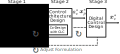
\includegraphics[width=0.6\textwidth]{../ch1/figures/stages2.pdf}
\caption{Proposed stages for complete dynamic system design.\label{fig:ch1:stages}}
\end{figure}

Allowing flexibility in all design domains can create a number of challenges that can limit how effectively one arrives at a suitable solution.
Here we adopt the design process proposed in Ref.~\cite{Deshmukh2015a} for complete dynamic system design that helps manage the complexity and uncertainty found in combined architecture, plant, and control design problems.
It is a three stage process shown in Fig.~\ref{fig:ch1:stages}.
We denote the plant architecture as $\glsfirst{architecture}_{\glsfirst{plant}}$ and associated plant variables as $\gls{x}_p$.
The control architecture is represented with $a_{\glsfirst{control}}$ and control variables $\bm{x}_c$ (and OLC variables as $\gls{olc}$).
The system-level objective function is represented by $\gls{objective}$.

% new paragraph
The first stage seeks to determine the optimal plant architecture by forgoing the specification of the control architecture.
Using a specific control architecture limits creative plant design exploration at early design stages \cite{Deshmukh2015a}.
Instead, OLC is used for the control among other potential uses.
OLC can replace some components or interfaces with optimal trajectories, reducing the design problem size while still providing an optimal solution \cite{Deshmukh2015a, Herber2014a, Allison2014b}.
In addition, OLC-based studies are particularly valuable at early design stages for gaining insights into upper system performance limits and dynamic behaviors and interactions that lead to system-optimal performance \cite{Allison2014a, Allison2013d,Son2010a, Schaala1993a, Mourik2009a, Karkee2010a}.
Furthermore, combined plant and control design, or co-design, will be used to determine the performance for each candidate plant architecture because it is a system-level optimization strategy \cite{Herber2017b, Fathy2003a, Allison2014a} that will allow fair comparisons between candidate plant architectures \cite{Bayrak2015a}.

\begin{figure}
\centering
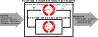
\includegraphics[width=0.8\textwidth]{../ch1/figures/outerinner2.pdf}
\caption{Stage 1 details.\label{fig:ch1:outerinner}}
\end{figure}

% new paragraph
The specifics for stage 1 are shown in Fig.~\ref{fig:ch1:outerinner}.
The inputs are the information about the system's operating environment, objectives, constraints, and a catalog of candidate components.
A nested optimization approach is used to handle the different variable types.
Here the outer loop will change the discrete (plant) architecture design variables while the inner loop determines the optimal performance by solving the continuous co-design problem for the candidate architecture. 

% new paragraph
Stage~2 in Fig.~\ref{fig:ch1:stages} seeks to determine the best control architecture given the optimized plant architecture from stage~1.
Similar to stage~1, a nested optimization approach can be used to vary the discrete control architecture decisions while the appropriate co-design problem is solved to determine the optimal performance for the candidate architecture.
For example, we could consider a basic feedback, hybrid \cite{Lygeros2008a}, or model predictive \cite{Borrelli2017a} controller architectures.
The final stage, stage~3, seeks to determine the digital controller design given the plant and controller architectures from the previous stages \cite{Landau2006a}.

% new paragraph
It might be necessary to iterate between the stages if unforeseen issues appear.
Information about these issues can be passed back to the previous stage and the problem formulation can be adjusted to address overlooked elements.
Additionally, in each of the stages, a sequence of problems may be posed and solved, each one informed by the results of the previous problem, moving toward greater levels of system specificity.

The theory and studies in this dissertation will primarily focus on design problems in stage~1, but it is important to understand the motivations behind these studies and how they fit into the entire design process.

%----------------------------------------------------------
\section{Solution Generation Challenges\label{sec:ch1:theorytools}}

There are a number of challenges associated with the design freedom found in combined architecture, plant, and control problems.
The complexity of individual problems can be quite significant, sometimes even rendering the problem intractable, unless this complexity is handled appropriately.  
Efficiently automating the key tasks in the solution generation process is essential to arriving at desirable solutions in a practical manner.
Here we highlight three important generation tasks: candidate architecture generation, model generation, and optimization problem generation.

%----------------------------------------------------------
\subsection{(Automated) Candidate Architecture Generation\label{sec:ch1:archgen}}

Exploring different architectures requires an appropriate conceptual framework that allows for modifications to the appropriate elements in the architecture.
A straightforward, commonly used representation is an adjacency matrix where the nonzero entries in the matrix represent connections between elements in the architecture.
Candidate architectures could be a different set of nonzero values in the adjacency matrix.
However, not all architecture representations are equally useful.
Some might produce many infeasible systems or too many candidates.
Others might produce many architectures with poor performance, or are not amendable to some optimization procedure.
An example alternative representation framework was developed for electrical circuits where a sequence of low-level instructions are used to generate a circuit \cite{Lohn1999a}.
These instructions iteratively add new elements to the circuit in  topologically different ways.
A manual alternative would include experts proposing candidate architectures, which may be appropriate in some cases, but often may not support comprehensive design space exploration.
In many traditional engineering design problems, the architecture is fixed so this abstract representation is not typically needed.

%----------------------------------------------------------
\subsection{(Automated) Model Generation\label{sec:ch1:modelgen}}

Given some architecture specification (e.g.,~a graph), we need to create a suitable model (some representation of the architecture that can predict performance and identify if constraints are satisfied) for use in the optimization problems described in Sec.~\ref{sec:ch1:process}.
Certain modeling methodologies support this task such as bond graph
modeling \cite{Borutzky2010a} or block diagram-based modeling \cite{matlab-simulink}. 
Other techniques have been developed for specific types of problems such as solid isotropic material with penalization for structural optimization \cite{Bendsoe2004a} and \glsfirst{MNA} for electrical circuits \cite{Ho1975a}.
Nevertheless, for many design problems, some investment will be needed to generate models efficiently and in an automated manner.
In traditional engineering design problems, the model is fixed for the given architecture, but can vary based on the plant/control design variables.

%----------------------------------------------------------
\subsection{(Automated) Optimization Problem Generation}

For different candidate architectures of the same design problem,  the optimization problem that predicts its performance may vary.
If the model is different, there may be different plant and control variables.
Different constraints may be present depending on the components in the architecture (e.g.,~we only need control actuator bounds if the component is present).
Since all problem elements (e.g.,~number and types of variables, objective function form, constraints, model) could change between architectures, forming and solving the optimization problem automatically is important for solution efficiency.
Understanding the general optimization problem structure for any candidate architecture is key so that it can be leveraged to find solutions faster and more robustly.
For some types of optimization problems, such as ones with infinite-dimensional constraints and variables, additional work is need to obtain (approximate) solutions.
Frequently, only a single optimization problem form needs to be posed and solved in traditional engineering design problems.

\section{Dissertation Overview\label{sec:ch1:overview}}

This introduction has provided a discussion on the combined architecture, plant, and control design problems including how this problem type can be used in the dynamic system design process and some potential challenges.
Due to the diverse design domains considered in this dissertation, a variety of methodologies are presented to manage different elements in the design process.
Chapters \ref{ch:2}--\ref{ch:5} focus on the development of these methodologies while Chapters \ref{ch:6}--\ref{ch:8} present detailed engineering design case studies that utilize the concepts.
A focus in the initial chapters is on the generality of the proposed approaches.
The frameworks presented are developed with specific consideration of what types of problems will fit under the proposed framework.

\begin{itemize}
% new paragraph, architecture
\item Chapter~\ref{ch:2} focuses on the task of representing and generating candidate architectures.
The theory and algorithms developed in this chapter are applicable to architecture problems where the architecture is representable by a colored graph built from a catalog of components.
A complete listing of all potential architectures under specific assumptions can be generated with this approach.
A number of enhancements to the algorithms presented in this chapter are detailed in Appendix~\ref{app:A}.

% new paragraph, co-design
\item Chapter~\ref{ch:3} focuses on a methodology for handling the other two design domains: combined plant and control design or co-design.
The general co-design problem formulation and optimality conditions are explained for both the simultaneous and nested solution strategies.
Due to a number of challenges associated with the optimality conditions, practical solution  considerations are discussed with a focus on the motivating reasons for using direct transcription in co-design.

% new paragraph, scaling
\item Chapter~\ref{ch:4} concentrates on scaling in dynamic optimization (a general class of problems found in Chapter~\ref{ch:3}). 
The necessary theory for scaling dynamic optimization formulations is presented and a number of motivating examples are shown. 
Scaling can be used to help facilitate finding accurate, generalizable, and intuitive information. The unique structure of dynamic optimization suggests that scaling can be utilized in novel ways to provide better analysis and formulations more favorable for efficiently generating the solution. 
A simpler, scaled problem is used to understand the general trends found in the results of the case study in Chapter~\ref{ch:7}, along with minor roles in the other two case studies.

% new paragraph, direct transcription
\item Chapter~\ref{ch:5} presents the direct transcription method for finding approximate solutions to dynamic optimization problems.
The method discretizes (in time) the infinite-dimensional quantities and creates a mathematical program that can be solved.
This method is an enabling method that allows solutions to be obtained for general co-design problems in Chapter~\ref{ch:4}.
A bulk of the chapter is focused on solving a particular subclass: linear-quadratic dynamic optimization problems.
These problems can be approximated with quadratic programs and be efficiently constructed and solved.
Problems with this structure are particularly important when the three domains are considered because many control problems may need to be solved, and an inefficient method could hinder the ability to explore the solutions.
The algorithms, sparsity patterns, and example codes are in Appendix~\ref{app:C}.
The case studies in Chapter \ref{ch:7} and \ref{ch:8} utilize this theory and codes to solve the control subproblem.

% new paragraph, passive analog circuits
\item Chapter~\ref{ch:6} presents an enumeration-based synthesis methodology for passive analog circuits by generating and evaluating all appropriate circuits.
Two design problems are considered: frequency response matching and low-pass filter realizability.
The circuit graphs (architectures) are generated using the methods described in Chapter~\ref{ch:2}.
This problem contains both architecture and plant design decisions.

% new paragraph, strain-actuated solar arrays
\item Chapter~\ref{ch:7} focuses on the design of strain-actuated solar arrays for spacecraft precision pointing and jitter reduction.
This problem has a variety of challenging plant and control design variables.
The nested co-design strategy described in Chapter~\ref{ch:3} is utilized, and the control subproblem is solved with the methods in Chapter~\ref{ch:5}.
The primary example from Chapter~\ref{ch:4} provides a number of insights into the results found in this case study.

% new paragraph, vehicle suspensions
\item Chapter~\ref{ch:8} is a case study that combines all three design domains with the design of vehicle suspensions.
The work from Chapters~\ref{ch:2}--\ref{ch:5} all contribute in addressing this complex design problem.
This chapter also includes a discussion of a general class of architecture, plant, and control design problems that utilize linear physical elements.

% new paragraph, conclusion
\item Chapter~\ref{ch:9} concludes the dissertation with an overall summary of the key points and identifies future research directions.

\end{itemize}

\begin{figure}[hb]
\centering
\includegraphics[width=0.65\textwidth]{../ch1/figures/outline2.pdf}
\caption[Dissertation content connections]{Dissertation content connections (dashed line indicates a narrower connection).\label{fig:ch1:outline}}
\end{figure}